
\begin{figure*}[t!]
    \centering
    \begin{subfigure}[b]{0.47\textwidth}
    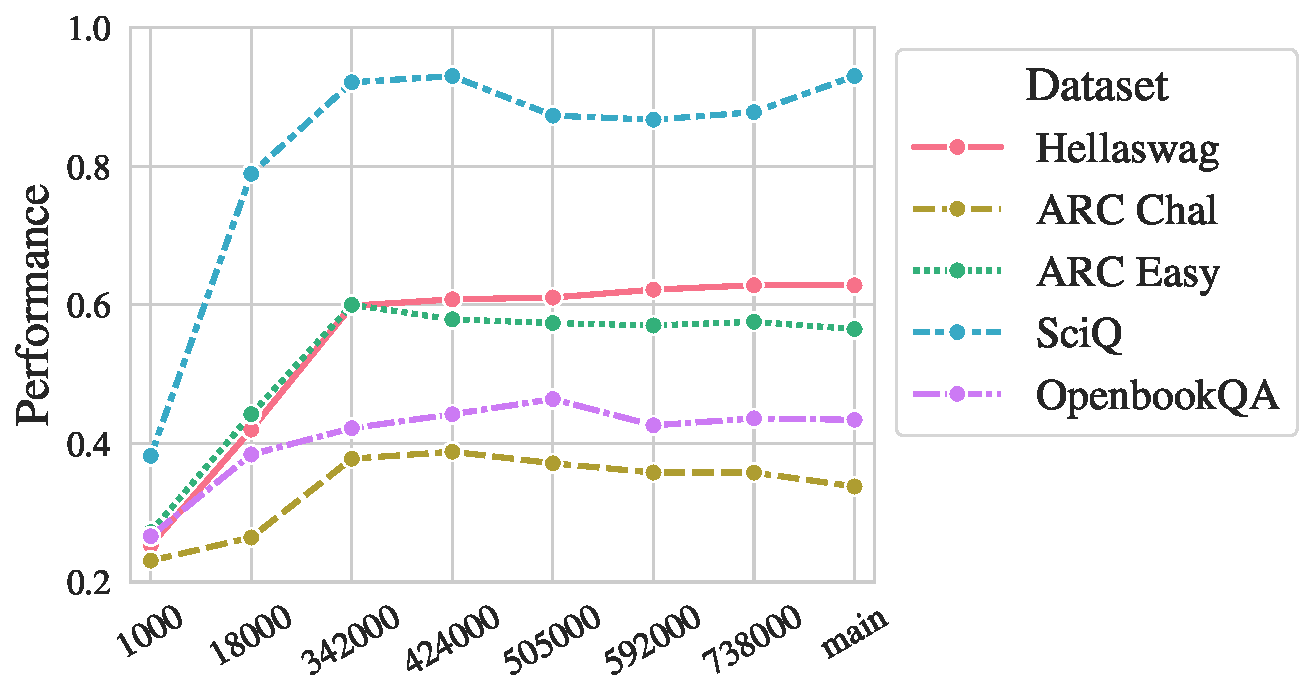
\includegraphics[width=\the\columnwidth]{figures/fig_files/base_improving.pdf}
        \caption{Learned during Pre-training.}
        \label{fig:base-eval-a}
    \end{subfigure}%
    ~ 
    \begin{subfigure}[b]{0.45\textwidth}
        \centering
    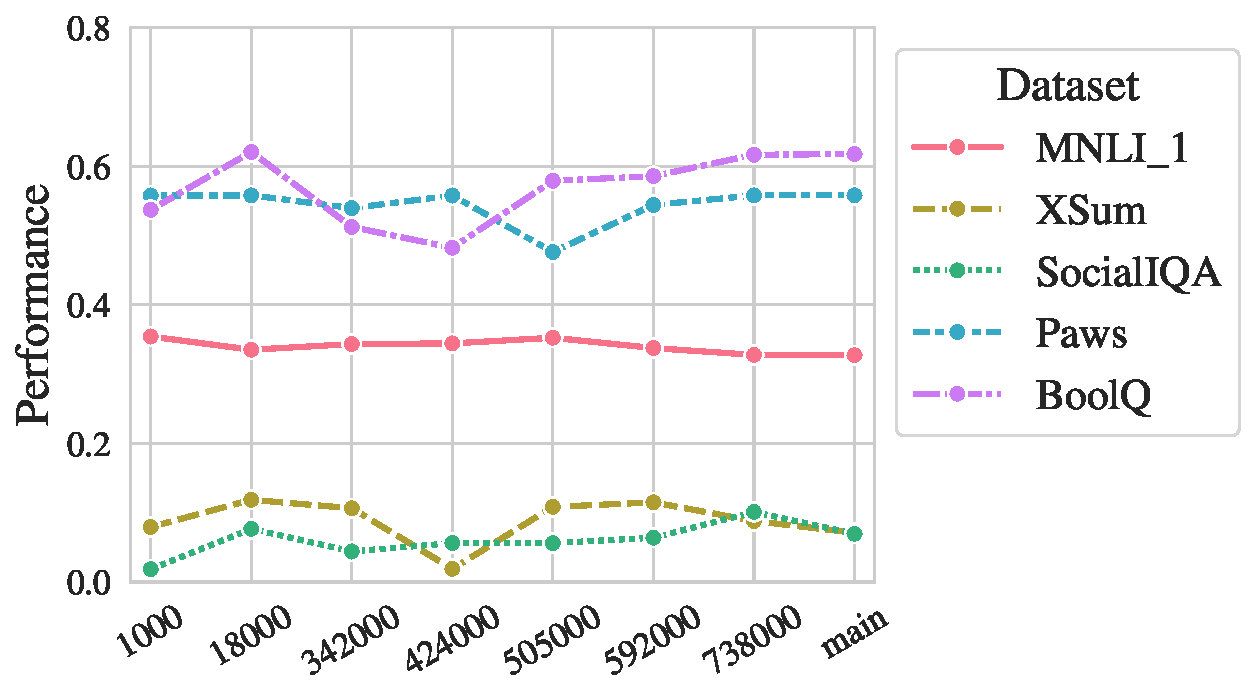
\includegraphics[width=\the\columnwidth]{figures/fig_files/base_notimproving.pdf}
        \caption{Never learned during pre-training.}
        \label{fig:base-eval-b}
    \end{subfigure}
    \caption{Few-shot performance on different pre-training steps.}
    \label{fig:base-eval}
\end{figure*}


\begin{figure}[t!]
    \begin{subfigure}[b]{0.5\textwidth}
    \centering
    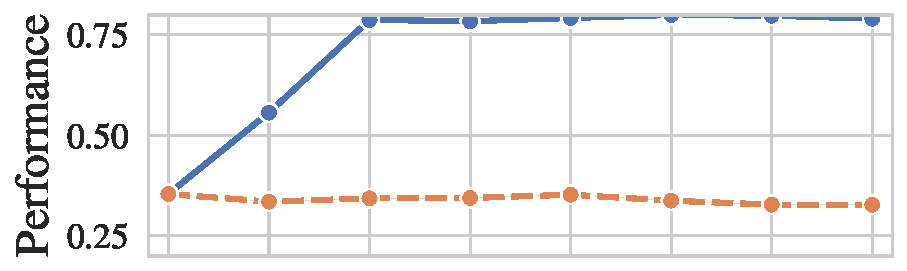
\includegraphics[width=0.8\columnwidth]{figures/fig_files/sft_evalmnli_matched-trainmnli_tight.pdf}
        \caption{MNLI Matched}
        \label{fig:subfig:improve}
    \end{subfigure}%
    \\
    \begin{subfigure}[b]{0.5\textwidth}
        \centering
    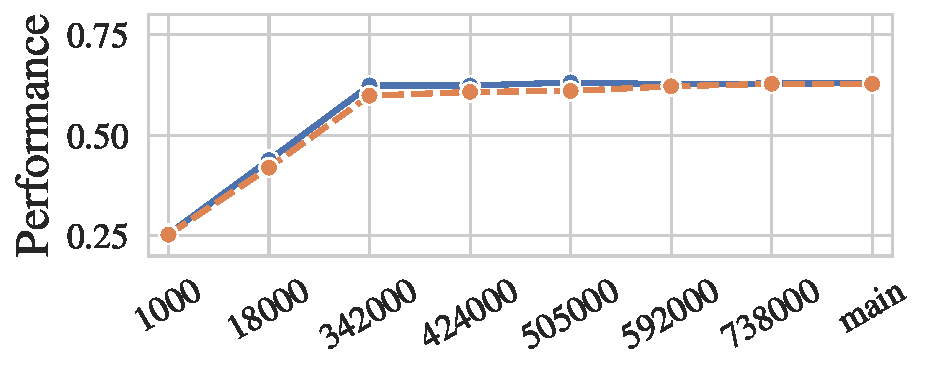
\includegraphics[width=0.8\columnwidth]{figures/fig_files/it_evalhellaswag_tight.pdf}
        \caption{Hellaswag}
        \label{fig:subfig:notimprove}
    \end{subfigure}
    \caption{Example of few-shot performance on different pre-training steps of the models that benefited (\ref{fig:subfig:improve}) and did not benefit from fine-tuning (\ref{fig:subfig:notimprove}). The \textcolor{snsblue}{\textbf{solid blue}} line represents the fine-tuned checkpoint, and the \textcolor{snsorange}{\textbf{dashed orange}} line represents the base checkpoint. The results of all datasets can be found in Figure~\ref{fig:sft-ckpt-perf} and Figure~\ref{fig:it-ckpt-perf}.}
    \label{fig:improve-and-notimprove-example}
\end{figure}
\begin{figure}[t]
    \centering
  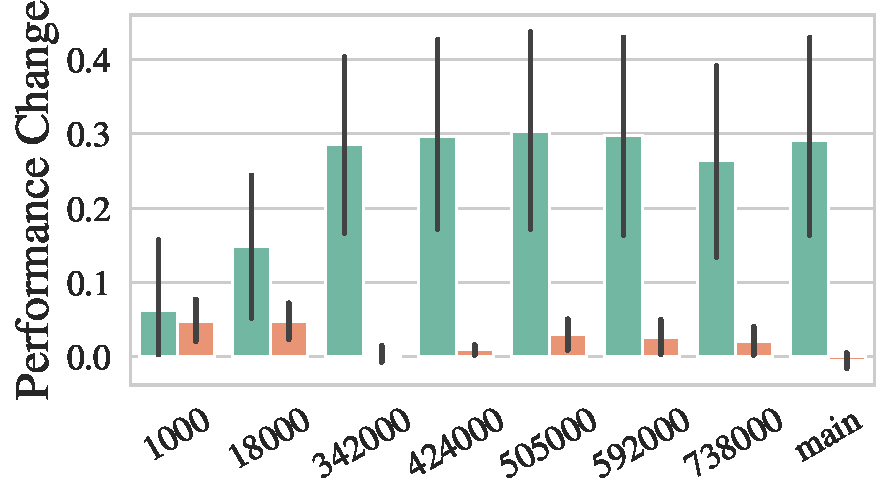
\includegraphics[width=0.84\columnwidth]{figures/fig_files/ptft_comparison_bar.pdf}
  \caption{Amount of performance increase brought by fine-tuning between tasks that model can solve in pre-training (\textcolor{snslightorange}{\textbf{mandarin orange}}) and tasks that the model could not solve until fine-tuning (\textcolor{snsgreen}{\textbf{sage green}}). The exact number of mean increase is shown in Appendix~\ref{sec:app:performance-numbers}.}
  \label{fig:finding:ptftcompare}
\end{figure}


\section{How does the model change across pre-training?}

\label{sec:finding:base-eval}
We begin our evaluation by considering how additional pre-training changes the BASE model. Typically, researchers track the value of the training or held-out loss during training. 
However, performance improvements on downstream tasks do not always follow the same trend with the loss curves \cite{groeneveld2024olmo}.

We evaluate the pre-trained checkpoints with few-shot examples, as models without alignment tend to do poorly in a zero-shot context.
Four shots are randomly sampled from the datasets, which are selected based on the highest performance shot amount reported in \citealp{yang2024unveiling}. 
The model's performance at each pre-training step is reported in Figure~\ref{fig:base-eval}.

Broadly speaking, our results suggest that all datasets fall into one of two groups. 
For the first group of datasets (Figure~\ref{fig:base-eval-a}), although the model shows clear improvement during the early stages of pre-training, performance levels off fairly early on and remains consistent. The dramatic improvements in the early stages of pre-training may result from larger steps in early optimization.
We find improvements stop increasing past step 342,000.
The second group (Figure~\ref{fig:base-eval-a}) shows tasks that are never learned during pre-training. 
Performance remains constant throughout the whole pre-training process. 
These datasets include MNLI, XSum, and BoolQ, and we found no difference between zero-shot and few-shot evaluations.
A natural hypothesis for this finding is potential data contamination in the pre-training data.
However, the evaluation datasets are selected based on the popularity of the task and the content of pre-training data. 
All datasets that experience improvement do not exist in the model's pre-training data \cite{soldaini2024dolma}, while the more likely leaked datasets (MNLI, XSUM) never gain an improvement during the pre-trining process.

Overall, these results reveal an interesting dichotomy. 
Some tasks can be learned during pre-training, while others are not. 
Next, we explore what exactly the model is learning regarding this second group of datasets during pre-training by exploring the fine-tuned models.

\section{Does more pre-training improve fine-tuning?}
\label{sec:finding:PTFT}
\citealp{groeneveld2024olmo} compares OLMo's performance on several tasks before and after fine-tuning the final checkpoint and finds that fine-tuning enables the model to do well on tasks for which the unaligned model does poorly. We observe (\sect{sec:finding:base-eval}) that while some datasets improved 
during pre-training, there is a group of datasets for which a pre-trained model does poorly.
Does the model learn anything that helps solve these tasks, and is fine-tuning required to do well on them? 
Alternatively, does the model learn useful information for these tasks but cannot express it without fine-tuning? In this section, we further explore this dataset dichotomy by examining fine-tuned checkpoints for each of the datasets. 


Our results appear in Figure~\ref{fig:improve-and-notimprove-example} and Figure~\ref{fig:finding:ptftcompare}. First, we consider those datasets where the pre-trained models do well (Figure~\ref{fig:base-eval-a}). 
These datasets do not improve with fine-tuning, suggesting whatever is learned during fine-tuning, which we discuss below, the model already gains the knowledge during pre-training. This effect is observed at all checkpoints; fine-tuning simply does not help.

However, a different story is observed for datasets that are not learned during pre-training. 
For these, fine-tuning yields significant improvements at every model checkpoint, with Figure~\ref{fig:finding:ptftcompare} showing the magnitude of improvement on these datasets compared to no improvement to the datasets already learned during pre-training.
Moreover, earlier checkpoints obtain more substantial gains from fine-tuning than later checkpoints.
The benefit of fine-tuning continues to increase until a certain threshold in pre-training steps is reached (approximately 424,000).

Figure~\ref{fig:improve-and-notimprove-example} shows representative plots comparing the performance of a pre-trained versus fine-tuned model at different checkpoints for two datasets (full list in Appendix~\ref{sec:app:per-ds-ckpt-figures}). 
For Hellaswag (learned during pre-training), fine-tuning does not benefit the model, even during early checkpoints when the model performs poorly on the task. 
Nevertheless, for MNLI (not learned during pre-training), fine-tuning dramatically improves the model. 
Interestingly, later checkpoints achieve better results after fine-tuning, even when the performance of the pre-trained model is unchanged. 
This suggests that the model is, in fact, learning important information during pre-training, but it cannot express that information without fine-tuning.


Our findings suggest that early stopping in pre-training will not be detrimental to downstream fine-tuning performance, and \textbf{the benefits of fine-tuning an LLM could exceed the benefits of continued pretraining}, which sheds light on the potential of cost-effective training paradigm with less pre-training.
However, it is difficult to directly identify such a stopping criteria without fine-tuning intermediate checkpoints; the improvement trend is invisible before fine-tuning the checkpoints.
Future work may reveal other signals of pre-training behavior that correlate with downstream task performance after fine-tuning.
Overall, when resource-intensive pre-trained LLMs are not available, fine-tuning models on models with less pre-training may be a reasonable practical choice for obtaining a high-quality model.


\section{Supervised Fine-Tuning: What does the model learn and forget?}
\label{sec:finding:what}
What exactly is the model learning during fine-tuning such that it shows abilities in pre-trained models for some tasks but provides no benefit for other tasks?
We analyze the supervised fine-tuning process to understand what is learned and what is forgotten. 
Specifically, we explore three dimensions: \textbf{task format, task transfer, and domain knowledge}.


\begin{figure*}[t!]
    \centering
    \begin{subfigure}[b]{0.36\textwidth}
    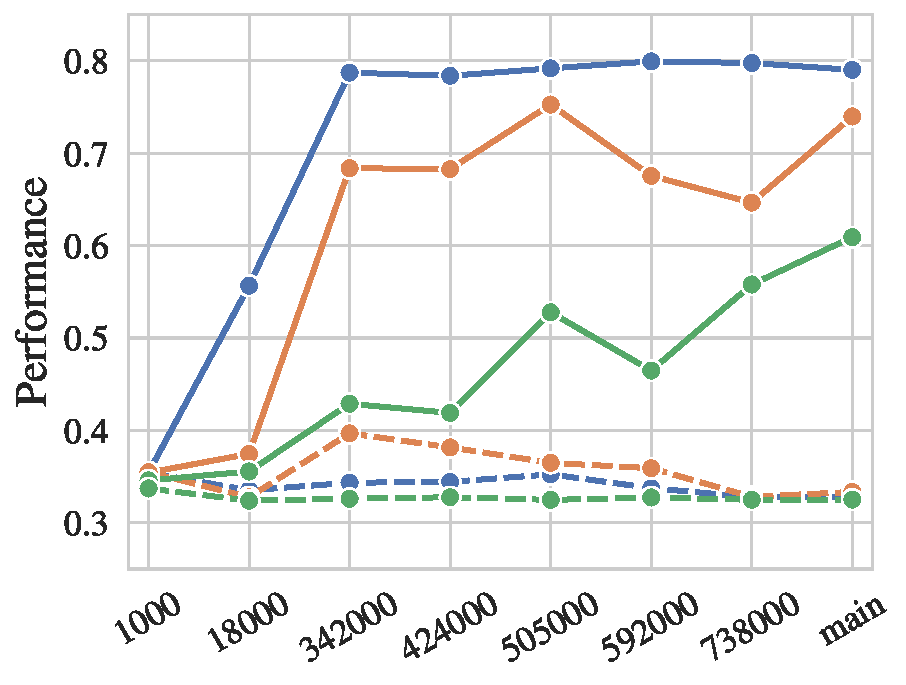
\includegraphics[width=\the\columnwidth]{figures/fig_files/task_format/task_format_evalmnli_matched-trainmnli.pdf}
        \caption{MNLI matched}
    \end{subfigure}%
    ~
    \begin{subfigure}[b]{0.51\textwidth}
    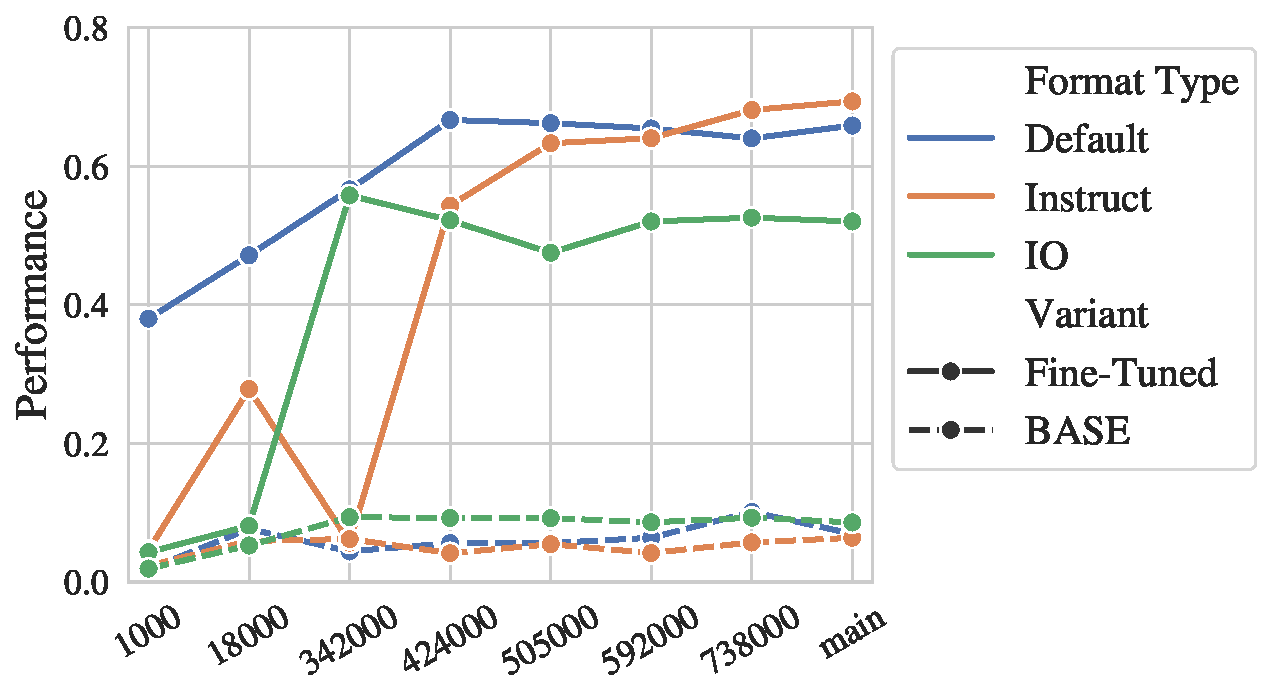
\includegraphics[width=\the\columnwidth]{figures/fig_files/task_format/task_format_evalsocialiqa-trainsocialiqa.pdf}
        \caption{SocialIQa}
    \end{subfigure}%

    \caption {Example of model performance with different task formats. The figure of all datasets can be found in Figure~\ref{fig:app:task_format}. }
  \label{fig:findings:task_format}
\end{figure*}
\subsection{Task Format}
\citealp{sclar2023quantifying} show that LLMs are extremely sensitive to prompt perturbation in few-shot settings. 
More broadly, extensive work on prompt engineering reveals the sensitivity of models to task format.
We hypothesize that fine-tuning fits the model to a specific task format, resulting in higher performance when the evaluation set matches this format. 
To test this hypothesis, we vary the task format to either match the training format, use a different format, or rely on instructions. 
We carefully construct three different prompt formats for the following settings. 1) 
\texttt{Default} is the same format used for training, where we expect the model to benefit from learning the task format;
2) In contrast, \texttt{IO} format reflects a common way of performing supervised fine-tuning by incorporating only unprocessed input and output;
3) \texttt{Instruct} uses a human-readable instruction template to format the input.
Table~\ref{tab:app:promptformat} shows an example of each format.
Checkpoint performance before and after fine-tuning is shown in Figure~\ref{fig:findings:task_format}.

In the early pre-training steps, aligning the task format with fine-tuning data seems to play a crucial role. 
The model does not yet have enough information to overcome the differences between the training and test formats.
However, when fine-tuned on later pre-training checkpoints, the model gradually becomes more flexible with different task formats, suggesting that model sensitivity to prompt formatting observed may be resolvable with more pre-training and a fine-tuning stage. In this view, fine-tuning teaches the model how to format a response for the task.


\subsection{Task Transfer}
Numerous studies examine model forgetting, where further model training causes improvements on some tasks but degradation on others \cite{mehta2023empirical}. 
We evaluate model forgetfulness by examining whether the model does worse on some tasks after fine-tuning for other tasks. 
Specifically, we divide our tasks into two types: classification and generation. 
We notate the training datasets as $D_{T}$ and the evaluation datasets as $D_{E}$. 
We represent the performance of a pre-trained model (BASE) on checkpoint $i$ as ${\text{Perf}}_{BASE}^i(d)$ where an evaluation dataset $d\in D_{E}$, and the performance of the i-th checkpoint fine-tuned on dataset $t \in D_{t}$ be $\text{Perf}_{t}^{i}(d)$. To normalize the effect caused by uneven performance across different datasets, we compute the mean ratio of change (MRC) in performance for each checkpoint as follows.
\begin{equation*}
\centering
    \resizebox{205pt}{!}{$\text{MRC} = \frac{1}{|D_{E}\setminus \{t\}|}\sum \limits_{\forall d \in D_{E}, d \neq t}{\frac{\text{Perf}_{t}^{i}(d) - {\text{Perf}}_{BASE}^i(d)}{\text{Perf}_{BASE}^i(d)}}$} 
\end{equation*}

Models fine-tuned on classification tasks and evaluated on generation tasks decrease on average 61.4\% compared to models that are never fine-tuned.
In contrast, models fine-tuned on generation tasks can still perform the same as the BASE model on classification tasks, with a 0.3\% MRC, which is not statistically significantly different from a 0\% change.
Our findings on all pre-training checkpoints align with the findings of \citet{yang2024unveiling} on the final checkpoint of LLAMA-7B.

Regardless of the pre-training stage, a model can maintain classification abilities when trained for generation, but it loses its generation abilities when trained for classification. 
This is perhaps not surprising given that classification tasks can be seen as a subset of generation, while the reverse is not true. 
The model follows a simplicity bias and thus is more likely to memorize simple classification tasks than generation tasks with an exponentially larger search space.
Additionally, since we evaluate the classification tasks based on the output logits and the base model performs randomly on the classification tasks, it is much easier for the models to maintain the same performance as the BASE models. 
Fine-tuning can cause a model to lose abilities when the desired fine-tuning behavior does not support those abilities.

\begin{figure}[t!]
    \begin{subfigure}[b]{0.5\textwidth}
    \centering
    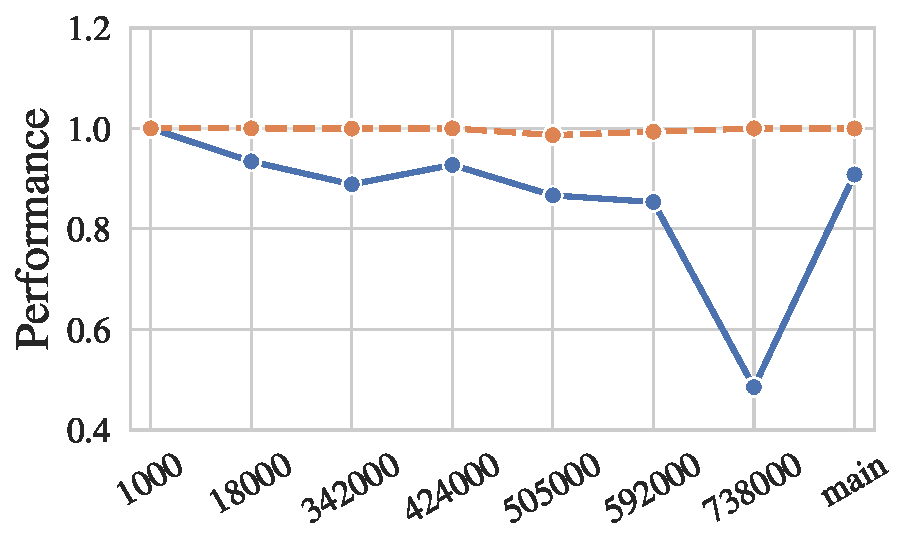
\includegraphics[width=0.7\columnwidth]{figures/fig_files/ood/sft_evalqqp-trainpaws_main_display.pdf}
        \caption{Paws $\rightarrow$ QQP}
        \label{fig:ood:detrimental}
    \end{subfigure}%
    \\
    \begin{subfigure}[b]{0.5\textwidth}
        \centering
    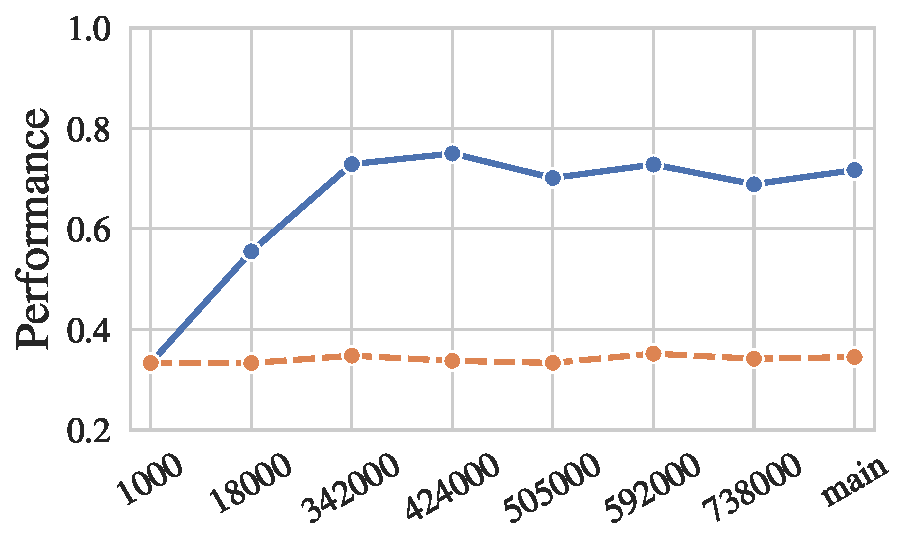
\includegraphics[width=0.7\columnwidth]{figures/fig_files/ood/sft_evalgpt3nli-trainmnli_main_display.pdf}
        \caption{MNLI $\rightarrow$ GPT3NLI}
        \label{fig:ood:beneficial}
    \end{subfigure}
    \caption{Example of out-of-domain performance for fine-tuned models. The \textcolor{snsblue}{\textbf{solid blue}} line represents the fine-tuned checkpoint evaluated on an out-of-domain dataset, and the \textcolor{snsorange}{\textbf{dashed orange}} line represents the base checkpoint where the model is not fine-tuned. Figure~\ref{fig:ood:detrimental} shows an example of fine-tuning hurting OOD performance, while Figure~\ref{fig:ood:beneficial} shows an example of fine-tuning boosting OOD performance as pre-traininng proceeds. }
    \label{fig:findings:ood}
\end{figure}
\begin{figure}[t]
\centering
  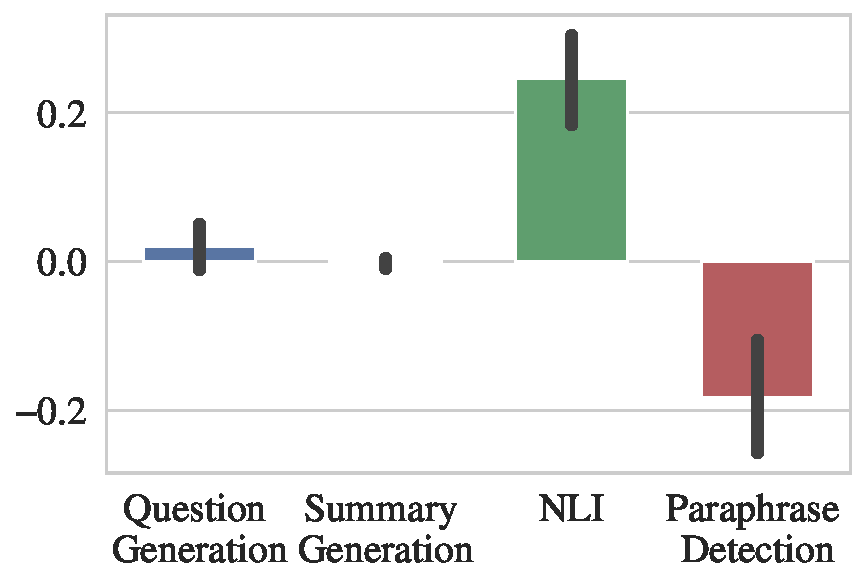
\includegraphics[width=0.65\columnwidth]{figures/fig_files/ood/weighted_ood_transfer_bar.pdf}
  \caption{Ratio of out-of-domain performance change for each task, averaged across checkpoints}
  \label{fig:finding:ood-by-data}
\end{figure}

\subsection{Domain Knowledge}
Finally, we explore how a model's generalization ability is affected by fine-tuning by inspecting whether the model forgets the domain knowledge it had before fine-tuning due to learning other abilities.
An example of OOD model performance is shown in Figure~\ref{fig:findings:ood}, and the mean change ratio by datasets is presented in Figure~\ref{fig:finding:ood-by-data}.

The model does not benefit equally from the in-domain fine-tuning: all NLI datasets experience a boost when fine-tuning on MNLI, while fine-tuning on Paws is detrimental to other paraphrase detection datasets.
This implies that both forgetting and learning are happening: the model learns to perform the task with in-domain knowledge, but it may, in turn, forget information more distant from what is learned in fine-tuning.
Questions remain, however, about whether there are different stages of learning and forgetting during fine-tuning and whether the model picks up different tasks in various stages, which requires further study of fine-tuning dynamics.

Overall, across these three lenses, we find that fine-tuning, although teaches a model how to perform a task, can sacrifice generalization abilities if such ability is not needed for the fine-tuned task. 
For some datasets learned with pre-training alone, the model can easily understand the task format, and the nature of the task is probably supported by the pre-training objective. 
For tasks that can only be learned with subsequent fine-tuning, the model may require additional examples to adapt to different task formats, or the task itself may be inconsistent with the pre-training objective.